\documentclass{../industrial-development}
\graphicspath{{10-configuration-problems/}}

\title{Проблемы управления конфигурацией и инструменты для их решения}
\author{Завойкин Алексей, ИТ-21 МО}
\date{}

\begin{document}

\begin{frame}
  \titlepage
\end{frame}

\begin{frame}{План лекции}
  \tableofcontents
\end{frame}

\section{Основные определения конфигурационного управления}

\begin{frame} \frametitle{Объект конфигурации (Configuration Item, CI):}
  
  \begin{itemize}
\item Исходные тексты
\item Скомпилированные программы
 \item Исходные коды программ
\item Документация
\item Элементы аппаратуры
 \item Процедуры и материалы обучения

  \end{itemize}
\end{frame}

\lecturenotes

При разработке программных систем создается множество взаимосвязанных объектов: требований, исходных текстов, объектных файлов, описаний тестов и т. п. — согласованные совокупности которых принято называть конфигурациями, а процесс поддержки их изменений и целостности в течение жизненного цикла проекта — управлением конфигурациями. Основная цель введения в проект процесса управления конфигурациями — предотвратить неконтролируемое развитие проекта и дать гарантии того, что все вносимые изменения будут учитываться и санкционироваться. Управление конфигурациями включает в себя процедуры по идентификации элементов проекта, по управлению изменениями и поддержке трассируемости объектов, а также деятельность по поддержке аудитов состояния и контролю статуса конфигурации.
Объект конфигурации (Configuration Item, CI): исходные тексты, скомпилированные программы, исходные коды программ, документация, элементы аппаратуры, процедуры и материалы обучения и т.п. — базовое понятие процесса управления конфигурациями Однако обычно под управление конфигурациями попадают только результаты проектной деятельности: программное обеспечение и сопутствующая документация, требования к интерфейсам и документация, выходные файлы, полученные при использовании инструментов проекта, технико-экономические документы и записи пользовательских требований, планы управления проектом, инструменты и руководства пользователя, записи об истории проекта, тест-планы, процедуры и отдельные тестовые примеры.~\cite{Standarts}

\begin{frame} \frametitle{Разработка интерфейса как часть цикла разработки ПО}
 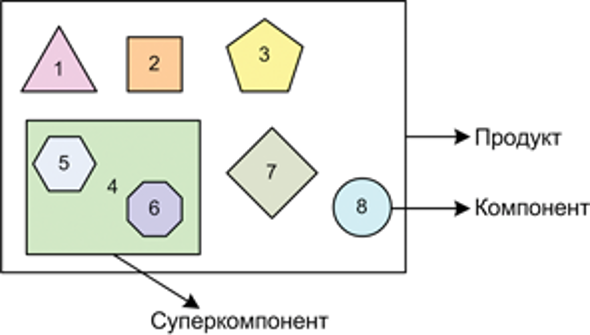
\includegraphics[width=\textwidth]{component}
\end{frame}

\lecturenotes

Получается, что CI – это любой файл в рамках проекта? Нет, нас интересуют только те файлы, которые необходимы и достаточны для создания конечного продукта для заказчика. Поэтому нам не нужны будут служебные и промежуточные файлы, генерируемые компиляторами, интерпретаторами и IDE. Нам также вряд ли будут интересны записи в блогах и форумах, проектная переписка и прочие продукты общения. Конечно, проектный документ по CM опишет средства общения внутри команды – но не более того.

К объектам, попадающим под действие CM, относятся и любые объекты, поставляемые вовне (инсталяторы, маркетинговые материалы и т.п.). Хоть их и можно получить из перечисленных выше рабочих продуктов, но конечный продукт, выдаваемый пользователю, также нуждается в идентификации.

Компонентная разработка и продуктовые линейки

Как же эти элементы конфигурации, атомарные единицы учета, организуются внутри проекта?

Складываются они вместе согласно архитектуре самого приложения. Ведь разработчики, как правило, стремятся уменьшить сложность производимых систем. С этой целью они раскладывают создаваемое на взаимосвязанные части – классы, компоненты, библиотеки, подсистемы и т.п. Упростим терминологию и в дальнейшем любые составные части создаваемых систем будем называть компонентами. CM же берёт эту организацию за основу и структурирует рабочие продукты соответствующим образом с помощью своих инструментов и политик.

Компоненты становятся новыми элементами конфигурации. Они становятся самостоятельными рабочими единицами, так же подлежащими единому контролю. Кроме того, они могут устанавливать даже собственный процесс разработки. CM’ные практики в этом случае нужны для того, чтобы эти отдельные блоки контролировать самостоятельным образом, получать промежуточные версии, стабилизировать и выпускать для интеграции в продукт более высокого уровня.

Итак, создаем систему, строим её из кирпичиков-компонентов. И нередка ситуация, когда одна система поставляется сразу в нескольких вариантах. За примерами далеко ходить не надо, взгляните на варианты поставки «Висты». И зачастую всё отличие разных вариантов/версий/редакций продуктов – всего в одном или нескольких компонентах, а то и вовсе в настройках. Как быть? Для этого создается то, что для простоты дальнейшего изложения будем называть продуктовыми линейками. Продуктовая линейка – это ответвление в истории развития продукта, дающее возможность изменять часть компонент независимо от других подобных ответвлений. (Здесь понятие «продукт» употребляется с маркетинговой точки зрения.
На схеме образно показан компонентный состав продукта. 1-8 — это компоненты, 4 — это «суперкомпонент», включающий в себя компоненты 5 и 6. В рамках интеграции продукта работа с ним ведется, как с обычным компонентом.
~\cite{Configurations}

\begin{frame} \frametitle{Разработка интерфейса как часть цикла разработки ПО}
 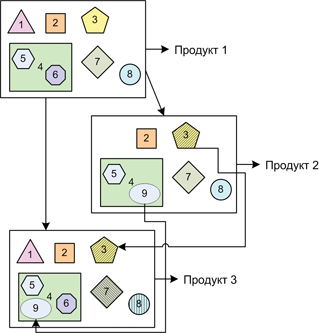
\includegraphics[width=\textwidth, height=7cm]{product}

\end{frame}

\lecturenotes

На схеме показано, как одни и те же компоненты могут быть использованы при работе с продуктовыми линейками. Например, имеется Продукт 1, состоящий из нескольких компонентов и суперкомпонента. На его основе производятся продукты 2 и 3.

Продукт 2 берет все те же компоненты, за исключением 1 и 6 — они исключаются из работы (или игнорированием соответствующих директорий, или выключением директив компиляции). В дополнение, изменяется компонент 3 — он становится 3' (штрих не проглядите). Также в единственный суперкомпонент добавляется новый компонент за номером 9.

Продукт 3 также берет за основу кодовую базу Продукта 1, однако берет в себя ещё и изменения из Продукта 2 — компоненты 9 и 3'. Также изменениям подвергаются компоненты 7 и 8, которые теперь называются 7' и 8' соответственно (да, тоже со штрихами).

Что в итоге? В итоге имеем несколько компонентов, интегрируемых одновременно в два-три разных продукта. Возьмем, к примеру, номер 2 – он неизменен во всех трёх продуктах. Напрашивается вывод – выпустить его один раз и просто «вставить» везде, где потребуют. Так и делается – компонентная команда в лице CM-инженера стабилизирует работу и передает на дальнейшую интеграцию трём «продуктовым» командам. Аналогично поступает CM-команда компонента 3’ – после внесения изменений поверх «предка» 3, полученный релиз компонента 3’ отдается в два продукта.

Причем использование одного компонента в разных продуктах – это не копирование исходников из директорий одного продукта в другой. Нет, смысл заключается именно в том, чтобы выпущенная конфигурация компонента находилась в системе контроля версий и все заинтересованные просто обращались к нему по мере включения в свой код.
~\cite{Configurations}
\begin{frame} \frametitle{В заметках о выпуске подробно указывается:}
  
  \begin{itemize}
\item Наименование нового релиза
\item Базис, на котором он основан
\item Изменения, вошедшие в релиз
\item Описание процедуры апгрейда рабочей копии системы
\item Описание процедуры самостоятельной подготовки исполнимых файлов

  \end{itemize}
\end{frame}

\lecturenotes

Стабилизация конфигурации – это процесс получения новой конфигурации из имеющихся промежуточных конфигураций. Для этого процесса также используются также термины «выпуск», «release» или «релиз». Результат стабилизации также может быть назван, в свою очередь, релизом или выпуском.

Например, есть основная конфигурация – версия продукта 1.0. Есть промежуточная конфигурация – разработанная девелопером новая «фича». Есть также 2 другие конфигурации – поправленные ошибки от двух других разработчиков. Стабилизацией в данном случае будет объединение результатов работы всех трех разработчиков и создание из них новой конфигурации, т.е. набора CI, которые образуют готовый продукт.

Полученная конфигурация проверяется на соответствие требованиям к составляющим её рабочим продуктам. Требования могут быть разнообразными, как правило, это количественные критерии качества. Скажем, с 3 девелоперами подобное требование к коду – это успешное прохождение 98 процентов регрессионных тестов. Код от всех разработчиков интегрируется, конфигурация стабилизируется, продукт собирается (например, отстраивается) и отдается на тесты.

Для релиза также делаются release notes. На русский этот термин переводится как «заметки о выпуске» или «дополнительные сведения» – так этот термин звучит в глоссарии Microsoft. Также может быть использовано «описание выпуска».
~\cite{Configurations}

\begin{frame} \frametitle{Baseline}
   \begin{block}{Baseline – это конфигурация, выбранная и закрепленная на любом этапе жизненного цикла разработки как основа для дальнейшей работы.}
  
 \end{block}
\end{frame}
	
	\lecturenotes
	Базовая конфигурация

Baseline – это конфигурация, выбранная и закрепленная на любом этапе жизненного цикла разработки как основа для дальнейшей работы. Переводом термина могут быть фразы «базовая конфигурация», «базовый уровень», «базовая версия» или «стабильная база». В дальнейшем будет преимущественно использован термин «базовая конфигурация».

Если вернуться обратно к нашему примеру про трёх разработчиков, то там стабилизированная конфигурация прошла оценку качества. То же самое обязательно и при выпуске базовой конфигурации. Менеджмент (тим-лид или SQA) смотрит на показатели качества, а также на другие факторы – например, на результаты инспекций кода или что-то ещё, что может вызвать сомнения. После чего принимает решение о том, что релиз должен быть взят за основу для работы всех остальных разработчиков, быть базой для разработки. Далее CM-инженер выполняет разного рода действия (например, навешивает метку и отстраивает код продукта) и выбранная конфигурация становится базовой. При этом она (как минимум, в виде исходников) выкладывается в открытый для всей команды доступ.

Возможен вариант, когда конфигурация не проходит по критериям качества и вообще не может быть использована для сборки конечного продукта. Например, продукт только начал разрабатываться и готов только код отдельных компонентов, да и у тех – заглушки вместо работающих функций. Нужно сделать конфигурацию основой работы для всей команды, но при этом миновать процедуру релиза – просто потому, что пока нельзя ничего собрать воедино. Такая конфигурация также имеет право быть использованной в качестве базовой, главное — четко обозначить имеющиеся ограничения по использованию в заметках о выпуске.

Любой выпуск базовой конфигурации обязательно снабжается заметками о выпуске. Участник команды, берущий подобную конфигурацию для работы, должен знать – от чего именно он будет отталкиваться в работе. Также надо знать, есть ли в новой конфигурации те новые функции или исправления ошибок, от которых может зависеть его работа. Не лишним будет также знать, нужны ли какие-то специальные процедуры апгрейда его экземпляра системы перед использованием новой базы для разработки. Вся перечисленная информация как раз дается в заметках о выпуске.

Во многих командах результаты интеграционной работы (появляющиеся релизы и базовые конфигурации) выкладываются в специально отведенное место – область релизов, или release area. Организация этой области и поддержание её в актуальном виде – задача CM-инженеров.
~\cite{Configurations}

	
\begin{frame} \frametitle{Baseline}
 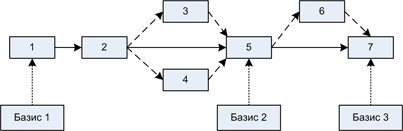
\includegraphics[width=\textwidth]{baseline}

\end{frame}

\lecturenotes

На схеме показан небольшой пример появления конфигураций во времени. Начальное состояние проекта – конфигурация 1. Она же является первым базисом, от которого будет идти дальнейшая разработка. Предположим, проект на начальной стадии. Через какое-то время появляется обновленная конфигурация 2. Разработка только началась и мы выпустили релиз, чтобы выдать команде хоть какую-то основу для дальнейшей работы. В ходе проверки выяснилось, что базой для работы этот выпуск служить не может – есть непонятные и противоречивые места.

Для их устранения группы разработки делают доработки. В результате них появляются конфигурации 3 и 4 – оба они разработаны на основе 2, но друг с другом они пока не согласуются, поскольку не включают изменения друг от друга. CM-инженер создает итоговую конфигурацию 5, сделанную на основе 2, 3 и 4. После проверки менеджмент дает отмашку – базовой конфигурации быть! По этому сигналу CM-команда выпускает этот релиз как официальную базовую конфигурацию и разработчики берут уже её за основу.

Далее история повторяется – группа разработки вносит изменения – появляется конфигурация 5. Её, в свою очередь, интегрирует CM-инженер и она получает номер 7. Он также становится официальной базой для разработки.
~\cite{Configurations}

\begin{frame} \frametitle{Конфигурация}
   \begin{block}{Конфигурация — любая структурированная совокупность объектов разработки программной системы, представленных в виде CI, или совокупность процессов и технологических цепочек проекта по разработке программной системы, описания которых также могут быть представлены в виде CI.}
  
 \end{block}
\end{frame}
	
	
	\lecturenotes
	При объединении объектов конфигурации образуется их конфигурация — любая структурированная совокупность объектов разработки программной системы, представленных в виде CI, или совокупность процессов и технологических цепочек проекта по разработке программной системы, описания которых также могут быть представлены в виде CI. Процесс управления конфигурациями в различных отраслях регламентируется международными и национальными стандартами: ГОСТ Р 51904, DO-178, AS9100, AS9006, ISO10007, ISO/IEC TR 15846, ISO/IEC 15408, IEEE 1042 и пр. При разработке высококритичных систем применение процесса управления конфигурациями строго обязательно — цена исправления дефектов в таких системах может быть очень высока.
~\cite{Standarts}

\begin{frame} \frametitle{Понятие воспроизводимости процесса}
  
  \begin{itemize}
\itemПроцесс является воспроизводимым, если продукция соответствует спецификации
\itemПроцесс является стабильным (управляемым), если на него влияют только общие причины вариабельности


  \end{itemize}
\end{frame}

\lecturenotes
Согласованный и воспроизводимый процесс. Используются всегда одинаковые процессы, независимо от того, о чем идет речь. (Фактически, целью должно стать разрешение вариаций, чтобы каждый проект мог стать успешным. Следовательно, постоянное использование одного и того же процесса и тот же объем процесса на протяжении всего проекта - это антишаблон, который приведет к провалу. Реальная задача - согласованность и воспроизводимость результатов.);

Воспроизводимость результатов. Адаптируемый процесс позволяет рабочей группе приспособиться к тактическим потребностям проекта. Благодаря этому рабочая группа получает поддержку и гибкость, которые необходимы ей для получения воспроизводимых результатов. Однако во многих случаях воспроизводимые результаты требуют некоторой адаптируемости в процессе, чтобы обеспечить соответствие тактическим требованиям; "воспроизводимость" в данном случае не может означать просто 100-процентно идентичное воспроизведение процесса, а, скорее, воспроизводимость фаз процесса, каждая из которых проходит через известный ряд шагов, результатов и показателей; 
~\cite{Instruments}

\section{Цели и процессы конфигурационного управления}
\begin{frame} \frametitle{Цели процесса управления конфигурациями}
 
	   \begin{block}{Цели процесса управления конфигурациями состоят в том, чтобы обеспечить:
		}
  		 \begin{itemize}
\item Определяемую и управляемую конфигурацию ПО на протяжении всего жизненного цикла
\item Целостность при тиражировании исполняемого объектного кода для производства ПО или, в случае необходимости, его повторной генерации для проведения исследований или модификации
\item Управление входными и выходными данными процесса в течение жизненного цикла, что гарантирует непротиворечивость и повторяемость работ в процессах

  \end{itemize}
 \end{block}
\end{frame}

\begin{frame} \frametitle{Цели процесса управления конфигурациями}
	   \begin{block}{Цели процесса управления конфигурациями состоят в том, чтобы обеспечить:}
  		 \begin{itemize}
			\item Контрольную точку для проверки, оценки состояния и контроля изменений посредством управления элементами конфигурации и определения базовой линии
		\item Контроль над тем, чтобы дефектам и ошибкам было уделено внимание, а изменения были зарегистрированы, утверждены и реализованы
\item Оценку соответствия программного средства требованиям
\item Надежное физическое архивирование, восстановление и сопровождение элементов конфигурации
  \end{itemize}
 \end{block}
\end{frame}

\lecturenotes
Стандарт ГОСТ Р 51904 был принят Госстандартом России в 2002 году и регламентирует требования к разработке и документированию встроенных систем. В нем процесс управления конфигурациями отнесен к группе интегральных процессов, необходимых для обеспечения качества выполнения процессов разработки и их выходных данных. Интегральные процессы выполняются одновременно с процессами разработки и обеспечивают непрерывную поддержку разработки. Основные цели процесса управления конфигурациями согласно ГОСТ 51904 состоят в следующем
~\cite{Standarts}

\begin{frame} \frametitle{Подпроцессы конфигурации}
  \begin{block}{Подпроцессами конфигурации являются:}
  		 \begin{itemize}
\item Установление набора правил, регламентирующих доступ к элементам конфигурации различных групп пользователей
\item Протоколирование всех действий по доступу к элементам конфигурации и их изменению
\item Определение базовой линии 
\item Архивирование конфигураций
  \end{itemize}
 \end{block}
\end{frame}


\lecturenotes
Процесс при этом разбит на несколько подпроцессов. При идентификации происходит однозначная маркировка каждого элемента конфигурации и последующих версий с целью установки базиса для управления и ссылок на элементы конфигурации. Для этого принимается схема идентификации, определяющая правила маркировки различных типов элементов конфигурации, их версии, ревизии, статуса. Подпроцесс контроля конфигурации состоит в установлении набора правил, регламентирующих доступ к элементам конфигурации различных групп пользователей, а также в протоколировании всех действий по доступу к элементам конфигурации и их изменению.
Следующим подпроцессом является определение базовой линии разработки с целью создания «моментального снимка» состояния конфигурации в заданный момент времени. Базовая линия может использоваться далее либо как отправная точка для создания новых конфигураций, либо для определения элементов системы, передаваемых для сертификации в сертифицирующий орган.
В процессе управления конфигурациями силами коллектива разработчиков и другими участниками проекта составляются отчеты о дефектах, содержащие описания несоответствий разрабатываемой системы требованиям либо несоответствия процессов разработки принятым стандартам. Управление отчетами о дефектах должно гарантировать, что качественно и в срок будут выполнены корректирующие действия, устраняющие дефекты.
Контроль изменений необходим для предотвращения спонтанной эволюции системы — все вносимые в нее изменения должны быть зарегистрированы, оценены, рассмотрены и утверждены. Такие изменения не нарушают целостности системы и конфигурации. Одновременно осуществляется архивирование конфигурации — это основной подпроцесс, гарантирующий, что все CI в конфигурации утверждены, а изменения в них — санкционированы. Это обеспечивается за счет разграничения прав доступа к CI и определения правил их изменения различными группами разработчиков. Разработчик не сможет получить доступ к CI, если этот доступ не был санкционирован.
~\cite{Standarts}

\begin{frame} \frametitle{Подпроцессы ведения отчетности}
\begin{block}{Подпроцессы ведения отчетности о состоянии конфигурации, необходимы для:}
  \begin{itemize}
\item Определения планов разработки, узких мест, установления сроков
\item Контроля загрузки ПО, в результате чего из CI создается конфигурация, предназначенная для выпуска и/или для загрузки во встраиваемую систему (этой конфигурации присваивается  номер и определяется аппаратура, на которой должна работать система)
\item Контроля среды жизненного цикла, дающего гарантию того, что все инструменты проекта идентифицируются, управляются, контролируются и могут быть получены из базы данных проекта
  \end{itemize}
	\end{block}
\end{frame}

\begin{frame} \frametitle{Конфигурационное управление}
 \begin{block}{Конфигурационное управление в программной инженерии — комплекс методов, направленных на:}
  \begin{itemize}
\itemСистематический учёт изменений, вносимых разработчиками в программный продукт в процессе его разработки и сопровождения 
\itemСохранение целостности системы после изменений
\itemПредотвращение нежелательных и непредсказуемых эффектов
\itemФормализацию процесса внесения изменений
  \end{itemize}
	\end{block}
\end{frame}

\lecturenotes
В целом, конфигурационное управление отвечает на вопрос: «Кто-то уже сделал нечто, как нам это воспроизвести?»
Изначально управление конфигурацией применялось не в программировании. Под конфигурацией понимался состав деталей конечного продукта и «взаимное расположение частей» физического изделия. Таким образом, конфигурацией можно управлять, контролируя документы, описывающие конечный продукт, требования к нему, всю его проектную и технологическую документацию.

\section{Процедуры конфигурационного управления}
\begin{frame} \frametitle{Процедуры управлений конфигурацией}
  \begin{block}{Процедуры управлений конфигурацией:}
  \begin{itemize}
\itemКонтроль исходного кода
\itemКонтроль требований проекта
\itemКонтроль документации
\itemКонтроль документации 
  \end{itemize}
	\end{block}
	\end{frame}

\lecturenotes
В связи с высокой динамичностью сферы разработки ПО, в ней конфигурационное управление особенно полезно. К процедурам можно отнести создание резервных копий, контроль исходного кода, требований проекта, документации и т. д. Степень формальности выполнения данных процедур зависит от размеров проекта, и при правильной её оценке данная концепция может быть очень полезна.

\begin{frame} \frametitle{Задача управления конфигурацией и её актуальность в промышленной разработке}
  
\end{frame}

\lecturenotes
Управление конфигурацией является основополагающей дисциплиной в определении того, каким образом управляются и контролируются рабочие материалы проекта, вносимые в них изменения и информация о состоянии отдельных задач и всего проекта в целом. Успех проекта в большой степени зависит от того, насколько хорошо построен процесс управления конфигурацией, который может как спасти проект, так и похоронить его, если сам процесс УК работает плохо. 

\begin{frame} \frametitle{Процедуры управлений конфигурацией}
  \begin{block}{Базовые процедуры управления конфигурацией:}
  \begin{itemize}
\itemДекомпозиция требований
\itemРевизия конфигурации
\itemАудит конфигурации
\itemКонтроль конфигурации
\itemУчет состояния конфигурации
  \end{itemize}
	\end{block}
\end{frame}

\lecturenotes
Проблема воспроизводимости процесса и подходы к её решению. 
Базовые процедуры управления конфигурацией
Итак, после определения требований, список остальных документов, составляющих конфигурационную спецификацию, определялся для каждого участниками проекта. Но как удостовериться в том, что эти документы создаются с нужным качеством и с достаточной степенью детализации?
Обычно используется метод декомпозиции требований (или «функциональной декомпозиции») – требования разбиваются на отдельные элементы и детализируются на следующем шаге разработки (дизайн). Затем детализация продолжается на следующем шаге и так далее до тех пор, пока не достигнут требуемый уровень детализации.
Другой способ – сравнение разрабатываемого документа с документами более высокого уровня, которые были утверждены ранее в процессе разработки. Для этой работы было использовано понятие «ревизия» (review) с добавлением слова «конфигурация». «Ревизия конфигурации» (configuration review ) представляет собой сравнение документа низкого уровня с предшествующим ему документом или документом верхнего уровня с тем, чтобы удостовериться, что документ нижнего уровня удовлетворяет всем требованиям, присутствующим в документе верхнего уровня, и нет никаких неожиданных добавлений. Это позволяет постепенно и аккуратно детализировать требования верхнего уровня в документах низкого уровня, уточняя конфигурационную идентификацию по мере разработки конфигурационного объекта.

Ревизия конфигурации используется также для того, чтобы проверить работоспособность продукта на основе документа соответствующего уровня. Например, ревизия исходного кода служит для того, чтобы удостовериться в том, что исходный код написан в соответствии с установленными правилами. Таким образом, ревизия конфигурации служит как для проверки правильности декомпозиции документов всех уровней, так и для проверки этих документов с точки зрения их соответствия правилам, шаблонам и форматам, используемым при создании такого рода документов.

Подобная техника проверки того, что продукт создается по установленным правилам и требованиям, используется при проведении «аудита конфигурации» (configuration audit ). Аудит конфигурации подобен процессу ревизии за исключением одной особенности – объектом приложения аудита является конфигурационный объект или конечный продукт, который сравнивается с документацией, составляющей его конфигурационную идентификацию. Объектом приложения ревизии являются отдельные документы.

Еще один способ гарантировать точность конфигурационной спецификации – иметь специальную группу (возможно, состоящую из одного специалиста), которая отслеживала бы все предлагаемые изменения продукта и отвергала или одобряла их. Такая деятельность получила название «контроль конфигурации» (configuration control)/ Группы, выполняющие функции контроля конфигурации обычно получают название «Группа контроля над изменениями» (Change Control Board) или «Группа контроля конфигурации» (Configuration Control Board, сокращенно CCB). Среди важных функций такой группы – контроль того, что все документы являются актуальными в каждый момент времени и того, что при внесении изменения сначала изменяются документы конфигурационной идентификации, а уже после – сам объект изменений (исходный код, модель и т.п.). Изменение объекта после изменения его описания выгодно еще и тем, что исполнитель, вносящий изменение в объект, будет иметь возможность ознакомиться с описанием этого изменения до начала работы.
Другой областью ответственности управления конфигурацией стала подготовка отчетности о состоянии продукта и состоянии утвержденных изменений на протяжении всего хода работ. Эта деятельность получила название «учет состояния конфигурации» (configuration status accounting)~\cite{Managing}

\begin{frame} \frametitle{Базовые концепции управления конфигурацией}
  \begin{block}{Базовые концепции управления конфигурацией:}
  \begin{itemize}
\itemДокументы создаются для описания продукта и являются средством управления конфигурацией продукта.
\itemИзменения в продукте контролируются посредством контроля изменений в документации.
\itemИзменения в продукте не производятся до тех пор, пока они не сделаны в документации.
\itemДо того, как быть реализованными в документации и продукте, изменения должны быть формально утверждены.
  \end{itemize}
	\end{block}
\end{frame}

\begin{frame} \frametitle{Базовые концепции управления конфигурацией}
  \begin{block}{Базовые концепции управления конфигурацией:}
  \begin{itemize}
\itemВсе изменения должны отслеживаться.
\itemКонфигурационные объекты (продукты), документы и их версии нумеруются и именуются единообразно и недвусмысленно (или уникально).
\itemВедется отчетность о состоянии изменений, документов и продуктов.
\itemКаждый документ периодически сравнивается с соответствующим ему документом верхнего уровня на предмет выявления несоответствий.
\itemПродукт в целом сравнивается со своим описанием (конфигурационной идентификацией) и должен этому описанию соответствовать.
  \end{itemize}
	\end{block}
\end{frame}

\lecturenotes
Используя введенную выше терминологию управления конфигурацией, эти концепции были сгруппированы в следующие четыре элемента управления конфигурацией:
	
Конфигурационная идентификация (концепция 1)
Контроль конфигурации (концепции 2, 3, 4, 5, 6)
Учет состояния конфигурации (концепция 7)
Ревизия и аудит конфигурации (концепции 8 и 9)
Такова была первоначальная концепция управления конфигурацией как для программных средств (software), так и для оборудования (hardware). Представленную здесь первоначальную терминологию дисциплины управления конфигурацией можно также найти в стандарте IEEE-STD-610. Далее будут рассмотрены стандарты, определяющие основные положения и терминологию управления конфигурацией.
Недостаточно четкое понимание терминологии управления конфигурацией, происходящее обычно из-за отсутствия формального обучения этой дисциплине, зачастую приводит к смещению концептуальных понятий и путанице в основополагающих принципах УК.
Так, например, основной элемент управления конфигурацией «конфигурационная идентификация» зачастую воспринимается в значении наименования или нумерации документа или продукта, что должно соответствовать понятию «идентификации документа» или «идентификации продукта». В то время как понятие «конфигурация» не относится к документу или продукту. Это понятие относится к содержанию документов, обозначая содержание технической документации, описывающей продукт. Кстати говоря, правила наименования и нумерации документов и продуктов относятся к следующему элементу УК – «контролю конфигурации», и называются «соглашением по наименованию и нумерации».
~\cite{Projects}
\begin{frame} \frametitle{Основные элементы управления конфигурацией}
 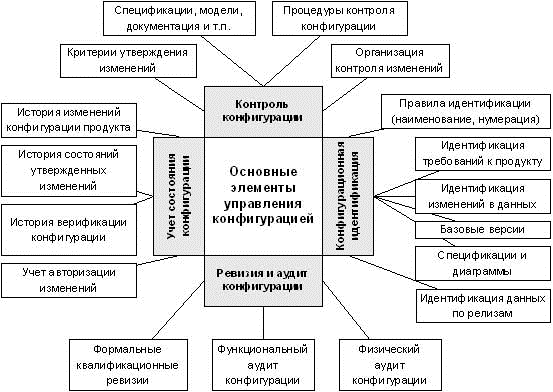
\includegraphics[width=\textwidth]{cmelements.png}
 \begin{block}{}
  
 \end{block}
\end{frame}

\lecturenotes

\begin{frame} \frametitle{Конфигурационная идентификация}
  \begin{block}{Конфигурационная идентификация основывается на следующих составляющих:}
  \begin{itemize}
\itemПравила идентификации и нумерации – что и каким образом идентифицируется
\itemИдентификация требований к продукту – каким образом идентифицируются требования к ПС
\itemИдентификация изменений в данных – каким образом идентифицируются изменения в данных
\itemБазовые версии – создаются для фиксации стабильных состояний системы и используются как кандидаты на релиз ПС
  \end{itemize}
	\end{block}
\end{frame}

\begin{frame} \frametitle{Конфигурационная идентификация}
  \begin{block}{Конфигурационная идентификация основывается на следующих составляющих:}
  \begin{itemize}
\itemСпецификации и диаграммы – документы, описывающие конфигурационную спецификацию ПС и диаграммы, используемые для этих же целей
\itemИдентификация данных по релизам – методы, позволяющие однозначно сопоставить элементы конфигурации ПС и их версии с определенным релизом ПС
  \end{itemize}
	\end{block}
\end{frame}

\lecturenotes

\begin{frame} \frametitle{Контроль конфигурации}
  \begin{block}{Контроль конфигурации включает:}
  \begin{itemize}
\itemКритерии утверждения изменений – определяют формальные критерии, на основании которых принимается решение об утверждении или отклонении предложенного изменения
\itemСпецификации, модели, документация и т.п. – все эти элементы конфигурации подвержены изменениям и находятся в сфере действия контроля конфигурации
\itemПроцедуры контроля конфигурации – утвержденные процедуры, которым должны следовать участники проекта
\itemОрганизация контроля изменений – организационная составляющая процесса, определяющая ответственность участников проекта при выполнении процедур контроля конфигурации
  \end{itemize}
	\end{block}
\end{frame}

\lecturenotes

\begin{frame} \frametitle{Учет состояния конфигурации}
  \begin{block}{Учет состояния конфигурации предполагает:}
  \begin{itemize}
\itemВедение истории изменений конфигурации продукта – определяет кто, когда и какие изменения делал;
\itemВедение истории состояний утвержденных изменений – показывает, как менялись состояния утвержденных изменений от момента утверждения и до момента завершения их отработки;
\itemВедение истории верификации конфигурации – хранит данные о всех проведенных верификациях и их результаты;
\itemУчет авторизации изменений – указывает на то, кто отвечает за сделанные изменения.
  \end{itemize}
	\end{block}
\end{frame}

\lecturenotes

\begin{frame} \frametitle{Ревизия и аудит конфигурации}
  \begin{block}{Ревизия и аудит конфигурации включает:}
  \begin{itemize}
\itemФормальные квалификационные ревизии – определяют соответствие элементов конфигурации предъявляемым к ним формальным требованиям, например, соответствие определенному шаблону документа
\itemФункциональный аудит конфигурации – определяет соответствие конфигурации ПС функциональным требованиям, предъявляемым к продукту
\itemФизический аудит конфигурации – определяет наличие или отсутствие отдельных элементов в составе конфигурации

  \end{itemize}
	\end{block}
\end{frame}

\section{Атрибуты конфигурационного управления}

\begin{frame} \frametitle{Автоматизация}
  \begin{block}{Автоматизация:}
  \begin{itemize}
\itemКаждый инструмент имеет специальный синтаксис и набор функций для написания сценариев автоматизации. 
\itemЯзык большинства инструментов похож на несколько упрощённый язык программирования
\itemДля создания более универсальных скриптов инициализации можно использовать переменные, циклы и условные выражения

  \end{itemize}
	\end{block}
\end{frame}

\lecturenotes

\begin{frame} \frametitle{Идемпотентность}
   \begin{block}{Идемпотентность:}
  \begin{itemize}
\itemСредства управления конфигурацией отслеживают состояние ресурсов, чтобы избежать повторения задач, которые были выполнены ранее. 
\itemК примеру, если пакет уже был установлен, инструмент не будет пытаться установить его снова. 
\itemСуть состоит в том, что после каждого запуска развёртывания система достигает необходимого состояния (или сохраняет его), даже если вы запускаете его несколько раз. 
\itemЭто и есть идемпотентное поведение (его можно применять опционально).

  \end{itemize}
	\end{block}
\end{frame}

\lecturenotes

\begin{frame} \frametitle{Подробные данные о системе }
  \begin{block}{Подробные данные о системе:}
  \begin{itemize}
\itemСредства конфигурационного управления предоставляют подробную информацию о системе, с которой они работают. 
\itemДоступ к таким данным можно получить с помощью глобальных переменных – так называемых фактов. 
\itemОни включают в себя сетевые интерфейсы, IP-адреса, операционные системы, распределение и многое другое. Каждый инструмент предоставляет индивидуальный набор фактов.
\itemИх можно использовать для создания универсальных и адаптивных сценариев и шаблонов, которые можно применить в нескольких системах.


  \end{itemize}
	\end{block}
\end{frame}

\lecturenotes

\begin{frame} \frametitle{Расширяемость }
  \begin{block}{Расширяемость: }
  \begin{itemize}
\itemЛюбой сценарий для управления конфигурацией можно индивидуализировать, подогнать под самые строгие требования и нужды конкретного сервера. 
\itemОднако часто возникает необходимость использовать одни и те же конфигурации (или их часть) на нескольких серверах. 
\itemБольшинство средств управления конфигурацией предоставляет возможность повторно использовать фрагменты сценариев в качестве модулей и плагинов.

  \end{itemize}
	\end{block}
\end{frame}

\lecturenotes

\section{Инструменты для управления конфигурацией}

\lecturenotes
Очень важно выбрать правильный инструмент, который хорошо подойдёт вашему серверу. Сегодня существует огромное количество средств управления конфигурациями разной сложности, каждое из которых предоставляет индивидуальный набор функций. Самыми популярными инструментами являются Chef, Ansible и Puppet.
~\cite{Instruments}
\begin{frame} \frametitle{Puppet}
  
  \begin{itemize}
\itemМодули могут быть написаны на ruby, или на более простом, производном от ruby языке
\itemКоманды Push позволяют применять изменения немедленно
\itemВеб-интерфейс поддерживает отчеты, инвентаризацию и управление узлами в реальном времени
\itemДетализированные отчеты о работе агентов и конфигурации узлов

  \end{itemize}
\end{frame}

\lecturenotes
Puppet Enterprise

Puppet считается наиболее используемым из четырех. Он наиболее полон с точки зрения возможных действий, модулей и пользовательских интерфейсов, представляя полную картину ЦОД, охватывая почти каждую операционную систему и предоставляя утилиты для всех основных ОС. Начальная установка относиельно проста, требует развертывания головного сервера и клиентских агентов на каждой управляемой системе.
Интерфейс командной строки позволяет загружать и устанавливать модули с помощью команды puppet. Затем требуются изменения в конфигурационных файлах, необходимые для настройки модуля под требуемую задачу, а клиенты, которые должны получить инструкции, получат их при следующем обращении к головному серверу, или через запрос от сервера, инициирующий процесс изменения немедленно.
Также имеются модули, с помощью которых выполняется настройка виртуальных и размещенных в «облаках» серверов. Все модули и конфигурации строятся с помощью встроеного, основанного на ruby, языка, или же на самом ruby. Это потребует некоторых знаний программирования, в дополнение к навыкам системного администрирования.
~\cite{Instruments}
\begin{frame} \frametitle{Enterprise Chef}
  
  \begin{itemize}
\item«Поваренные книги» и рецепты используют всю мощь ruby
\itemЦентрализованные, основанные на JSON массивы данных позволяют скриптам заполнять переменные во время работы
\itemВеб-интерфейс позволяет вести поиск и учет узлов, просматривать их активность, применять «поваренные книги» и роли
  \end{itemize}
\end{frame}

\lecturenotes
Chef похож на Puppet с точки зрения общей концепции, в нем также имеется головной сервер и агенты, установленные на управляемых узлах. В дополнение к головному серверу, установка Chef также требует рабочей станции, для управления им. Агенты могут быть установлены с рабочей станции с помощью утилиты knife, которая использует протокол SSH для развертывания, облегчая бремя установки. После этого, управляемые узлы аутентифицируются с головным при помощи сертификатов.

Конфигурация Chef тесно связана с системой управления версиями Git, поэтому знание того, как работает Git необходимо для работы. Также как и Puppet, Chef основан на ruby, поэтому потребуется и знание этого языка. Как и в случае с Puppet. Модули могут быть загружены или написаны «с нуля», после чего установлены на управялемые узлы, в соответствии с требуемыми настройками.

В отличие от Puppet, у Chef пока нет хорошо реализованной функции push, хотя доступна бета-версия кода. Это означает, что агентов должны быть настроены на периодическую синхронизацию с головным сервером, и немедленное применение изменений невозможно.

Пользовательский веб-интерфейс функционален, но не предоставляет возможности модифицировать конфигурации. Он не так полон, как веб-интерфейс Puppet Enterprise, уступает в построении отчетов и некоторых других функциях, но позволяет вести учет оборудования и организацию узлов.
Как и у Puppet, у Chef большой набор модулей и рецептов настроек, преимущественно на ruby. По этой причине, Chef хорошо подходит для инфраструктур, ориентированных на разработку.
~\cite{Instruments}
\begin{frame} \frametitle{AnsibleWorks Ansible}
  
  \begin{itemize}
\itemМодули могут быть написаны почти на любом языке
\itemНе требуются агенты на управляемых узлах
\itemВеб-интерфейс позволяет настраивать пользователей, команды и оборудование, применять сценарии
\itemОчень просто настраивается и запускается

  \end{itemize}
\end{frame}

\lecturenotes
Ansible больше похож на Salt, чем на Puppet или Chef. Ansible фокусируется на оптимизации и скорости, и не требует установки агентов на управляемые узлы — все функции производятся по SSH. Ansible написан на python, в отличие от Puppet и Chef, основанных на ruby.

Установка Ansible может быть выполнена путем клонирования Git-репозитория на головной сервер. Вслед за этим, узлы, над которыми требуется управление добавляются в конфигурацию Ansible, и авторизованные ключи SSH «привязываются» к каждому узлу, относясь к пользователю от имени которого будет запускаться Ansible. Как только это сделано, головной сервер может соединяться с узлами по протоколу SSH и выполнять все необходимые задачи. Для работы с системами, не позволящими доступ с правами суперпользователя (root) по SSH, Ansible использует учетные данные, позволяющие выполнять действия от имени суперпользователя с помощью команды sudo.

Ansible может использовать Paramiko — реализацию протокола SSH2 на языке python, или стандартную реализацию SSH, но есть также ускоренный режим, для более быстрой и широкомасштабной коммуникации.

Ansible может быть запущен из командной строки без использования конфигурационных файлов для простых задач, таких как проверка, что некий сервис запущен, или для обновления триггеров и перезагрузки. Для более комплексных задач, конфигурационные файлы создаются с помощью YAML и называются «сценарии» (playbook). В них могут быть использованы шаблоны для расширения функциональности.

В Ansible есть набор модулей, которые могут использоваться для управления различными системами, равно как и «облачными» инфраструктурами, такими как Amazon EC2 и OpenStack. Дополнительные модули могут быть написаны на практически любом языке программирования, при условии, что вывод будет в формате JSON.

Веб-интерфейс доступен в виде AnsibleWorks AWX, но напрямую не связан с интерфейсом командной строки. Это значит, что элементы конфигурации, заданные через командную строку, не появятся в веб-интерфейсе до тех пор, пока не будет запущен цикл синхронизации. Вы можете использовать встроенную утилиту для этого, но необходимо запланировать ее регулярный запуск. Сам по себе веб-интерфейсе достаточно функционален, но не такой полный, как интерфейс командной строки, таким образом вы либо будете переключаться между обоими, либо же просто использовать командную строку. 
~\cite{Instruments}
\begin{frame} \frametitle{SaltStack Enterprise}
  
  \begin{itemize}
\itemКонфигурационные файлы могут быть простыми YAML-шаблонами или скриптами на pyhton и PyDSL
\itemМожет связываться с клиентами через SSH или с помощью локально установленных агентов
\itemВеб-интерфейс позволяет просматривать запущенные задачи, статус подчиненных узлов и позволяет выполнять комнады на клиентах
\itemКрайне хорошо масштабируется

  \end{itemize}
\end{frame}

\lecturenotes
Salt схож с Ansible в том, что основан на командной строке. Он использует метод push для связи с клиентами. Он может быть установлен через Git или через систему управления пакетами на головном сервере и клиентах. Клиент делает запрос к головному серверу, и если тот дает разрешение, позволяет управлять данным узлом с помощью агента (в терминах Salt — minion).

Salt может связываться с клиентами по протоколу SSH, но масштабируемость значительно расширяется за счет клиентских агентов. Также, Salt включает асинхронный файловый сервер для ускорения обслуживания агентов, позволяя создавать хорошо масштабируемые системы.

Как и в случае Ansible, вы можете отдавать команды, такие как как запуск сервисов или установка пакетов агентам напрямую из командной строки, или можете использовать конфигурационные файлы в формате YAML (state), для обработки комплексных задач. Также есть централизовано размещенные наборы данных (pillar) к которым имеют доступ конфигурационные файлы во время работы.

Вы можете запросить информацию о конфигурации — такую как версия ядра или детальную информацию о сетевом интерфейсе — напрямую от агентов через командную строку. Агенты могут также задаваться через использование элементов инвентаря, называемых «зернами» (grain), позволяющими легко передавать команды на определенные сервера, безотносительно к настроенным группам. Например, одной командой можно отправить запрос к агентам, расположенным на серверах с определенной версией ядра.

Как и предыдущие продукты, Salt предоставляет большое количество модулей для разнообразного программного обеспечения, операционных систем и «облачных» сервисов. Вспомогательные модули могут быть написаны на языках python или PyDSL. Salt предоставляет возможность управлять и Windows-узлами, равно как и Unix, но больше расчитан на системы Unix и Linux.

Веб-интерфейс Salt — Halite — слишком новый и не полный, как пользоветельские интерфейсы других систем. С его помощью можно просматривать системные журнал сообщений и статус управляемых узлов, а также имеется возможность выполнять на них команды. Этот иснтурмент активно разрабатывается, и обещает значительные улучшения, но пока это голый «скелет» и содержит много ошибок.

Самое большое преимущество Salt — масштабируемость и гибкость. У вас может быть несколько уровней головных серверов, организующих связанную струкутру, для обеспечения распределения нагрузки и увеличения отказоустойчивости. Головные сервера верхнего уровня могут управлять нижестоящеми в иерархии и их подчиненными узлами. Другое преимущество — одноранговая система обмена сообщениями, позволяющая подчиненным узлам задавать вопросы головным, а те могут получать ответы от других серверов для завершения картины. Это может быть полезным, если даные для завершения настройки узла находятся в базе данных реального времени. 
~\cite{Instruments}


\begin{thebibliography}{99}

\bibitem{Configurations} \href{https://special.habrahabr.ru/kyocera/p/67839/}{Конфигурации и baselines}

\bibitem{Standarts} \href{https://www.osp.ru/os/2013/07/13037353/}{Стандарты процесса управления конфигурациями}

\bibitem{Article} \href{https://www.ibm.com/developerworks/ru/library/kroll_ambler/index.html}{Передовые методы управления разработкой с минимальными затратами}

\bibitem{Instruments} \href{https://habrahabr.ru/post/211306/}{Стандарты процесса управления конфигурациями}

\bibitem{Managing} \href{http://cmcons.com/articles/CC_CQ/konfiguratsionnoe_upravlenie_proektami_razrabotki_programmnogo_obespechenija/}{Конфигурационное управление проектами разработки программного обеспечения}

\bibitem{Projects} \href{http://citforum.ru/SE/quality/configuration_management/}{Конфигурационное управление проектами разработки программного обеспечения}
\end{thebibliography}

\end{document}
%%% Local Variables: 
%%% mode: TeX-pdf
%%% TeX-master: t
%%% End: 
